% \begin{savequote}[75mm]
%  Here, we seek equipment to tame this gorgon’s head with reflection.
% \qauthor{\citet{chapman2010gentle}}
% \end{savequote}

\chapter{Background}
\label{background}

\epigraph{Here, we seek equipment to tame this gorgon’s head with \gls{reflection}.}{\citet{chapman2010gentle}}

\section{CertiCoq}

Traditionally, a compiler is a program that reads code in the \emph{\gls{source language}} from a file, translates it to the \emph{\gls{target language}}, and writes the resulting code to a file. The language the compiler itself is implemented in is called the \emph{\gls{host language}}.
The host and source languages are often different languages. For example, the Elm and PureScript compilers are implemented in Haskell. For some compilers, the host and the source languages are the same, and they can compile themselves, these are called \emph{self-hosting compiler}s. The Glasgow Haskell Compiler~\cite{jones1993glasgow,marlow2004glasgow}, the Rust compiler~\cite{matsakis2014rust}, and more recently the Idris 2 compiler~\cite{brady2021idris} are examples of such compilers.

Let us take a look at how CertiCoq fits into this general picture. Colloquially CertiCoq is called ``a compiler for Coq in Coq''~\cite{certicoq}, yet the input method and the pipeline of CertiCoq differ from traditional compilers. As opposed to most compilers, CertiCoq is not an independent program; it was implemented as a Coq plugin. It does not take a file as an input; it takes a definition name and runs as a command in a Coq session:

\newcommand{\listsum}{\hyperref[code:listsum]{\fn{list\_sum}}}
\vspace{.1in}
\begin{SaveVerbatim}{E}
\kw{Definition} \listsum{}\label{code:listsum} : \ty{nat} :=
  \fn{List.fold_left} (\kw{fun} \bn{x} \bn{y} => \bn{x} \fn{+} \bn{y}) (\fn{List.repeat} \dt{1} \dt{100}) \dt{0}.
\end{SaveVerbatim}
\tocoq{\UseVerbatim{E}}

\begin{SaveVerbatim}{E}
\listsum{} is defined.
\end{SaveVerbatim}
\fromcoq{\UseVerbatim{E}}

\vspace{.1in}

\begin{SaveVerbatim}{E}
\kw{CertiCoq Compile} \listsum{}.
\end{SaveVerbatim}
\tocoq{\UseVerbatim{E}}

\begin{SaveVerbatim}{E}
\kw{list_sum.c} is generated.
\end{SaveVerbatim}
\fromcoq{\UseVerbatim{E}}




% \begin{Verbatim}
% \kw{Definition} \fn{list_sum} : \ty{nat} :=
%   \fn{List.fold_left} (\kw{fun} \bn{x} \bn{y} => \bn{x} \fn{+} \bn{y}) (\fn{List.repeat} \dt{1} \dt{100}) \dt{0}.
  
% \kw{CertiCoq Compile} \fn{list_sum}.
% \end{Verbatim}

Notice how the user first creates a Coq definition, and then a special \gls{Vernacular} command takes the name of this definition and compiles it. Can we call this compiling Coq? What does it mean to compile Coq anyway?

The part of Coq that we will consider consists of three languages: \textbf{\gls{Gallina}}, the term language based on the Calculus of Inductive Constructions~\cite{coquand1988inductively}, \textbf{\gls{Ltac}}, the domain-specific language for proofs and decision procedures, and \textbf{\gls{Vernacular}}, the collection of commands through which we can send queries and requests to the Coq system. These languages can even appear in the same definition. Here is an example that creates the natural number $2$, accompanied with a proof that $2$ is less than $5$:

\begin{Verbatim}
\kw{Definition} \fn{less_than_5} : \ty{sig} (\kw{fun} (\bn{n} : \ty{nat}) => \bn{n} \ty{<} \dt{5}).
\kw{Proof}. \tc{exists} \dt{2}. \tc{auto}. \kw{Defined}.
\end{Verbatim}

Here, \kw{Definition} is a \gls{Vernacular} command for making a new definition. The type of this definition is a function application term in \gls{Gallina}, that states that the definition is a sigma type (i.e.\ a dependent pair) containing a \ty{nat} and a proposition that \ty{nat} is less than \dt{5}. 
In the next line, that is followed by the \kw{Proof} \gls{Vernacular} command, which signals that the definition will be written in \gls{Ltac}. Indeed, there are two \gls{Ltac} tactics, the first one of which provides the witness of existence, namely \dt{2}. The second one automatically satisfies the goal of type \code{\dt{2} \ty{<} \dt{5}}. When the \gls{Vernacular} command \kw{Defined} is run, the \gls{Ltac} tactics construct a \gls{Gallina} term that satisfies this type. The goal here is simple enough that the \tc{auto} tactic suffices. For more complicated proofs, we would either have to use more tactics or use more complicated decision procedures. In order to see the proof term \gls{Ltac} generates, we can ask Coq to print the definition:

\vspace{.2in}
\begin{SaveVerbatim}{E}
\kw{Print} \fn{less_than_5}.
\end{SaveVerbatim}
\tocoq{\UseVerbatim{E}}

\begin{SaveVerbatim}{E}
\fn{less_than_5} = 
     \dt{exist} (\kw{fun} \bn{n} : \ty{nat} => \bn{n} \ty{<} \dt{5}) \dt{2} (\dt{le_S} \dt{3} \dt{4} (\dt{le_S} \dt{3} \dt{3} (\dt{le_n} \dt{3})) : \dt{2} \bn{<} \dt{5})
     : \{ \bn{n} : \ty{nat} | \bn{n} \ty{<} \dt{5} \}
\end{SaveVerbatim}
\fromcoq{\UseVerbatim{E}}

This term could have been written by hand, but it would take longer, while here running the \tc{auto} tactic generates it automatically, and it still works even if the numbers change. In other words, \gls{Ltac} scripts are interpreted at compile time to generate \gls{Gallina} terms. We will go deeper into the capabilities of \gls{Ltac} in \autoref{ltac}.

With this in mind, it would be more accurate to say CertiCoq compiles parsed and type-checked \gls{Gallina} terms into C.

\section{Inductive Types}

\Gls{inductive type}s are a mechanism to define custom data types in Coq.
They are a generalization of algebraic data types you find in mainstream typed functional programming languages like Haskell and ML.\footnote{Not to be confused with \emph{generalized algebraic data types}~\cite{cheney2003first} (GADTs), another generalization of algebraic data types influenced by inductive types, but a less expressive one. There is much larger literature on adding mechanisms to these languages to approximate \gls{inductive type}s, but that is not the topic of this dissertation.}
\newpage

Most values that we will inspect or generate in Coq will be values of \gls{inductive type}s. Their generality requires us to be precise about our terminology, therefore it will be helpful to revise the terms we use to refer to different parts of an \gls{inductive type}. Here is the classic example of an \gls{inductive type}, the vector type, which is a kind of list indexed by its length:

\renewcommand{\vec}{\hyperref[code:vec]{\ty{vec}}}
\newcommand{\vnil}{\hyperref[code:vec]{\dt{vnil}}}
\newcommand{\vcons}{\hyperref[code:vec]{\dt{vcons}}}
\begin{figure}[H]
\label{code:vec}
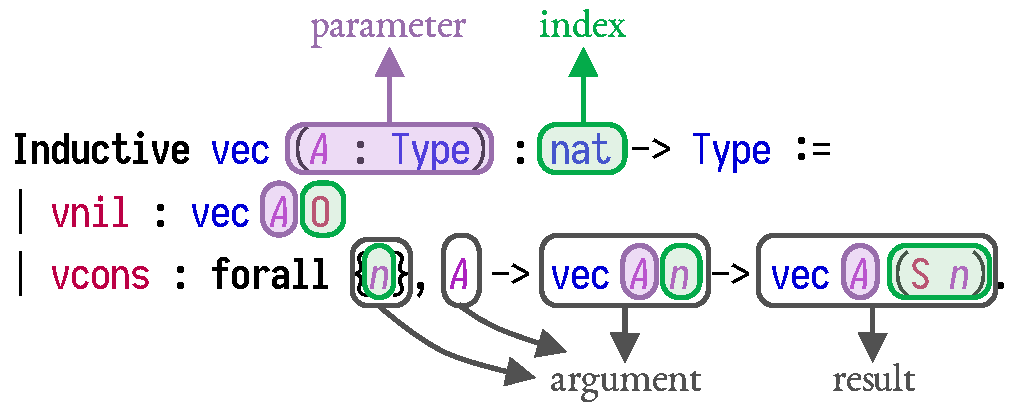
\includegraphics[scale=.59]{figures/inductive.pdf}
\centering
\caption{The definition of the \ty{vec} type in Coq.}
\end{figure}

% \begin{Verbatim}
% \kw{Inductive} \ty{vec} (\bn{A} : \ty{Type}) : \ty{nat} -> \ty{Type} :=
% | \dt{vnil} : \ty{vec} \bn{A} \dt{O}
% | \dt{vcons} : \kw{forall} \bn{n}, \bn{A} -> \ty{vec} \bn{A} \bn{n} -> \ty{vec} \bn{A} (\dt{S} \bn{n}).
% \end{Verbatim}

The code above defines a type \vec{} with two \emph{\glspl{data constructor}}: \vnil{} and \vcons{}. While \vec{} is the name of the inductive type, it doesn't have the type \ty{Type}, unlike a type like \ty{nat}. This is because \vec{} itself needs to take arguments. In other words, \vec{} is a \emph{\gls{type constructor}}. When the word ``constructor" is used alone, it refers to data constructors. The term ``\gls{data constructor}" is only used in contrast to type constructors.

The first of \vec{}’s arguments is an example of a \emph{\gls{parameter}}, and the second is an example of an \emph{\gls{index}}~\cite{dybjer1994}. Both \gls{parameter}s and \glslink{index}{indices} are arguments to the return type of the \gls{inductive type}. \Gls{parameter}s are written before the colon in the type signature of the \gls{inductive type} being defined, while indices come after. \Gls{parameter}s must remain consistent across all constructors' return types, while indices can vary. It is worth noting that all the return types in \vec{} have \bn{A} as the first argument, but the second argument varies between \dt{O} or \Verb|\dt{S} \bn{n}|. Thanks to this variation, the \vec{} type can be indexed with different list lengths.

Notice that \vnil{} takes no arguments, whereas \vcons{} takes three. The first argument that \vcons{} takes is named \bn{n}, while the other two arguments remain unnamed. This argument is named because the return type depends on it, whereas no type depends on the other two arguments. The type of this argument, \ty{nat}, can be omitted here since the type checker can infer it based on the type of \vec{}.

\paragraph*{Implicit and Explicit Arguments} The curly braces around \bn{n}, the first argument of \vcons{}, tell the Coq type checker that this argument is \emph{implicit}, which means this argument will be skipped in a normal application of \vcons{}, and the Coq type checker will try to infer it depending on the context.

\vspace{.2in}
\begin{SaveVerbatim}{E}
\kw{Check} \dt{vcons}.
\end{SaveVerbatim}
\tocoq{\UseVerbatim{E}}

\begin{SaveVerbatim}{E}
\dt{vcons}
     : \bn{?A} -> \ty{vec} \bn{?A} \bn{?n} -> \ty{vec} \bn{?A} (\dt{S} \bn{?n})
\kw{where}
\bn{?A} : [ |- \ty{Type}]
\bn{?n} : [ |- \ty{nat}]
\end{SaveVerbatim}
\fromcoq{\UseVerbatim{E}}

By adding \code{@} in front of a function or inductive type name, we can turn all implicit arguments in the type into explicit arguments:

\vspace{.2in}
\begin{SaveVerbatim}{E}
\kw{Check} @\dt{vcons}.
\end{SaveVerbatim}
\tocoq{\UseVerbatim{E}}

\begin{SaveVerbatim}{E}
@\dt{vcons}
     : \kw{forall} (\bn{A} : \ty{Type}) (\bn{n} : \ty{nat}), \bn{A} -> \ty{vec} \bn{A} \bn{n} -> \ty{vec} \bn{A} (\dt{S} \bn{n})
\end{SaveVerbatim}
\fromcoq{\UseVerbatim{E}}


\paragraph*{Inspecting Inductive Values}

Values of \gls{inductive type}s can be inspected by \kw{match} expressions. The programmer can write functions that contain \kw{match} expressions (and ones that do not) using the \kw{fun} keyword in \gls{Gallina} or the \kw{Definition} keyword in \gls{Vernacular}, as we have seen in the \listsum{} example. Recursive functions, however, need to be defined using the \kw{fix} keyword in \gls{Gallina} or the \kw{Fixpoint} keyword in \gls{Vernacular}:

\begin{Verbatim}
\kw{Fixpoint} \fn{vlength} \{\bn{A} : \ty{Type}\} \{\bn{n} : \ty{nat}\} (\bn{xs} : \vec{} \bn{A} \bn{n}) \{\kw{struct} \bn{xs}\} : \ty{nat} :=
  \kw{match} \bn{xs} \kw{with}
  | \vnil{} => \dt{O}
  | \vcons{} \bn{x} \bn{xs'} => \dt{S} (\fn{vlength} \bn{xs'})
  \kw{end}.

\kw{Definition} \fn{vmap} :=
  \kw{fix} \fn{vmap} \{\bn{A} \bn{B} : \ty{Type}\} \{\bn{n} : \ty{nat}\} 
           (\bn{f} : \bn{A} -> \bn{B}) (\bn{xs} : \vec{} \bn{A} \bn{n}) \{\kw{struct} \bn{xs}\} : \vec{} \bn{B} \bn{n} :=
    \kw{match} \bn{xs} \kw{with}
    | \vnil{} => \vnil{}
    | \vcons{} \bn{x} \bn{xs'} => \vcons{} (\bn{f} \bn{x}) (\fn{vmap} \bn{f} \bn{xs'})
    \kw{end}.
\end{Verbatim}

Here, we define two recursive functions. The first function, \fn{vlength} computes the length of a \vec{}. The second function, \fn{vmap} transforms all the elements of a \vec{} by applying the higher-order function \bn{f}.

In these examples, \fn{vlength} is defined using \kw{Fixpoint}, and \fn{vmap} is defined using \kw{fix}. In practice, top-level recursive functions are usually defined using \kw{Fixpoint}. The \kw{fix} syntax is usually reserved for when we have to write or generate \gls{Gallina} terms, or when we have to define recursive auxiliary functions within other functions.

\section{Metaprogramming Facilities}

A simple definition of \gls{metaprogramming} is the generation or analysis of programs by other programs. By this broad definition, C macros~\cite{stallman1987c} are \gls{metaprogramming}, JavaScript's \fn{eval} is \gls{metaprogramming}, even replacing text in code before compilation counts as \gls{metaprogramming}. \Gls{metaprogramming} comes in many different shapes and colors. 

In this thesis, we will use MetaCoq, a homogeneous generative \gls{metaprogramming}~\cite{hgmp} system for Coq, and \gls{Ltac}, a tactic language for Coq proofs. We will also later develop our own \gls{metaprogramming} abstractions that are based on these two systems.

\subsection{MetaCoq}
\label{metacoq}
MetaCoq is a project formalizing Coq in Coq, and it comes with a quoting mechanism for Coq~\cite{templatecoq, sozeau2020metacoq}. It provides \gls{primitive}s in Coq that can use and manipulate \gls{Gallina} terms and types based on a deeply embedded description of \gls{Gallina} terms, which can also be viewed as abstract syntax trees of \gls{Gallina} terms within \gls{Gallina}.

Here we see an example of a \emph{\gls{quotation}}, i.e. converting an expression into a deeply embedded description, i.e. the \ty{term} type in MetaCoq. 

% \kw{Check} <% \dt{true} %>.
\vspace{.2in}
\begin{SaveVerbatim}{E}
\kw{MetaCoq Run} (\fn{tmQuote} \dt{true} \fn{>>}\fn{=} \fn{tmPrint}).
\end{SaveVerbatim}
\tocoq{\UseVerbatim{E}}

\begin{SaveVerbatim}{E}
\dt{tConstruct}
  \{| \fn{inductive_mind} := (\dt{MPfile} [\dt{"Datatypes"}; \dt{"Init"}; \dt{"Coq"}], \dt{"bool"})
   ; \fn{inductive_ind} := \dt{0} |\} \dt{0} \dt{[]} : \ty{term}
\end{SaveVerbatim}
\fromcoq{\UseVerbatim{E}}

The description of the term \dt{true} above tells us that \dt{true} is the zeroth constructor of the type \ty{bool}, which is located in the \code{\ty{Coq}.\ty{Init}.\ty{Datatypes}} module.

For top-level quotations, we often use the \code{<\% ... \%>} syntax, defined as a simple Coq notation using the primitive tactic from MetaCoq:

\vspace{.2in}
\begin{SaveVerbatim}{E}
\kw{Check} <\% \fn{andb} \%>.
\end{SaveVerbatim}
\tocoq{\UseVerbatim{E}}

\begin{SaveVerbatim}{E}
\dt{tConst} (\dt{MPfile} \dt{[}\dt{"Datatypes"}; \dt{"Init"}; \dt{"Coq"}\dt{]}, \dt{"andb"}) \dt{[]})
  : \ty{term}
\end{SaveVerbatim}
\fromcoq{\UseVerbatim{E}}

The description of the term \fn{andb} tells us that \fn{andb} is a constant definition that is located in the \code{\ty{Coq}.\ty{Init}.\ty{Datatypes}} module.

Here is an example of an \emph{\gls{unquotation}} (also called \emph{antiquotation} or \emph{splice} in the literature), converting a deeply embedded description into an expression.
We have the \ty{term} description of the variable referring to the logical ``and'' operator for Boolean values. By unquoting it, we can obtain the actual \fn{andb} function.

\vspace{.2in}
\begin{SaveVerbatim}{E}
\kw{MetaCoq Run} (\fn{tmUnquoteTyped} _ 
               (\dt{tConst} (\dt{MPfile} \dt{[}\dt{"Datatypes"}; \dt{"Init"}; \dt{"Coq"}\dt{]}, \dt{"andb"}) \dt{[]})
             \fn{>>}\fn{=} \fn{tmPrint}).
\end{SaveVerbatim}
\tocoq{\UseVerbatim{E}}

\begin{SaveVerbatim}{E}
\fn{andb}
\end{SaveVerbatim}
\fromcoq{\UseVerbatim{E}}

For top-level unquotations, we often use the \code{\~{}( ... )} syntax, defined as a simple Coq notation using the primitive tactic from MetaCoq.


\newcommand{\TemplateMonad}{\hyperref[code:TemplateMonad]{\ty{TemplateMonad}}}
This is quite similar to systems like untyped\footnote{A template \gls{metaprogramming} system makes \emph{code fragments} first-class values. An \emph{untyped} template \gls{metaprogramming} system would give these code fragments the same type, such as the \ty{term} type in MetaCoq or the \ty{Exp} type in Template Haskell. A \emph{typed} template \gls{metaprogramming} system would give code fragments types based on the code in the fragment, such as \code{.<\dt{1}\fn{+}\dt{2}>. : \ty{int code}} in MetaML~\cite{taha2000metaml}.} Template Haskell (TH)~\cite{sheard2002template}. Both systems have a deeply embedded description type for expressions (\ty{Exp} for TH and \ty{term} for MetaCoq), a monadic interface for primitive actions (\ty{Q} for TH and \TemplateMonad\label{code:TemplateMonad} for MetaCoq), and a language primitive to run them (\code{\$(...)} splicing in TH and the \kw{MetaCoq Run} \gls{Vernacular} command in MetaCoq).

The primary features of MetaCoq we use are
\begin{enumerate}[nosep]
\item generating terms
\item generating definitions and type class instances
\item generating proof obligations
\item inspecting inductive types
\end{enumerate}
and we want to show examples of these in this section.


\paragraph*{Generating Terms}

Let us start with generating terms. The classic example of generative \gls{metaprogramming} systems is generating a specialized power function~\cite{sheard2001, taha2004, coutts2004, rompf2012, stucki2018}. This example is useful for illustrating the capabilities of a typed \gls{metaprogramming} system, and how well it can handle quasiquoting and scoping. As of the time this thesis is written, a dependently typed MetaML-style \gls{metaprogramming} system is an active research area and an unsolved problem for a full language~\cite{kawata2019dependently, xie2022staging}.


In the most naive form, you would write the power function as such:
\begin{Verbatim}
\kw{Fixpoint} \fn{naive_pow} (\bn{exponent} : \ty{nat}) (\bn{base} : \ty{nat}) : \ty{nat} :=
  \kw{match} \bn{exponent} \kw{with}
  | \dt{0} => \dt{1}
  | \dt{S} \bn{exponent'} => \bn{base} * \fn{naive_pow} \bn{exponent'} \bn{base}
  \kw{end}.
\end{Verbatim}

Observe that this function is recursive, but not tail recursive. One way we can use MetaCoq to optimize it to generate a power function specialized to its exponent. Such a function would allow us to have a non-recursive power function for a fixed exponent, such as \linebreak\code{\kw{fun} \bn{x} => \bn{x} \fn{*} (\bn{x} \fn{*} \bn{x})} that takes a number to its 3rd power. Here is a function that produces the deeply embedded description of such a function, given an exponent:

\newcommand{\makespecializedpow}{\hyperref[code:makespecializedpow]{\fn{make\_specialized\_pow}}}
\label{code:makespecializedpow}
\begin{Verbatim}
\kw{Definition} \makespecializedpow (\bn{exponent} : \ty{nat}) : \ty{term} :=
  \kw{let} \kw{fix} \bn{aux} (\bn{exponent} : \ty{nat}) (\bn{base} : \ty{term}) : \ty{term} :=
    \kw{match} \bn{exponent} \kw{with}
    | \dt{0} => <% \dt{1} %>
    | \dt{S} \bn{exponent'} => \dt{tApp} <% \fn{Nat.mul} %> [\bn{base}; \bn{aux} \bn{exponent'} \bn{base}]
    \kw{end}
  \kw{in} \dt{tLambda} \{| \fn{binder_name} := \dt{nNamed} \dt{"n"}; \fn{binder_relevance} := \dt{Relevant} |\}
             <% \ty{nat} %>
             (\bn{aux} \bn{exponent} (\dt{tRel} \dt{0})).
\end{Verbatim}


Now we can call the specialized power function generator with a specific exponent, \unquote{} the result, and observe the generated function term:

\vspace{.2in}
\begin{SaveVerbatim}{E}
\kw{Check} ~(\makespecializedpow{} \dt{3}).
\end{SaveVerbatim}
\tocoq{\UseVerbatim{E}}

\begin{SaveVerbatim}{E}
\kw{fun} \bn{n} : \ty{nat} => \bn{n} \fn{*} (\bn{n} \fn{*} (\bn{n} \fn{*} \dt{1})) : \ty{nat} -> \ty{nat}
\end{SaveVerbatim}
\fromcoq{\UseVerbatim{E}}

Notice that this specialized power function cubes the input nonrecursively, unlike the \fn{naive\_pow} function. Therefore, our initial goal has been achieved.

\paragraph*{Generating Definitions and Type Class Instances}

The function term generated by \makespecializedpow{} is not made into a definition yet. Ideally, the programmer would generate a definition specialized for a particular exponent and reuse it. Now, let us generate a definition using MetaCoq.

\begin{Verbatim}
\kw{Definition} \fn{generate_specialized_pow} (\bn{exponent} : \ty{nat}) : \TemplateMonad{} \ty{unit} :=
  \bn{name} <- \fn{tmFreshName} (\fn{append} \dt{"pow"} (\fn{string_of_nat} \bn{exponent})) ;;
  \bn{fn} <- \fn{tmUnquoteTyped} (\ty{nat} -> \ty{nat}) (\makespecializedpow{} \bn{exponent}) ;;
  \fn{tmDefinition} \bn{name} \bn{fn} ;;
  \fn{ret} \dt{tt}.
\end{Verbatim}

This function takes an exponent, such as 3, and generates a function named \fn{pow3}, defined as the function term generated by \makespecializedpow{} above:

\vspace{.2in}
\begin{SaveVerbatim}{E}
\kw{MetaCoq Run} (\fn{generate_specialized_pow} \dt{3}).
\kw{Compute} (\fn{pow3} \dt{2}).
\end{SaveVerbatim}
\tocoq{\UseVerbatim{E}}

\begin{SaveVerbatim}{E}
\dt{8} : \ty{nat}
\end{SaveVerbatim}
\fromcoq{\UseVerbatim{E}}

In this thesis, we will use Coq's type classes~\cite{sozeau2008first} as a way of organizing generated data, therefore it is useful to see an example use of MetaCoq with type classes.

Type classes, as defined in Haskell literature, usually are indexed by other types, and they are used for overloading a single function name for different types. Type classes in Coq are built upon dependent records. Like \gls{inductive type}s, they can have any kind (not just types) of \gls{parameter}s.
Here we can overload a single function name for different \ty{nat}s used as fixed exponents.

\begin{Verbatim}
\kw{Class} \ty{Pow} (\bn{exponent} : \ty{nat}) : \ty{Type} :=
  \{ \fn{pow} : \kw{forall} (\bn{base} : \ty{nat}), \ty{nat} \}.

\kw{Instance} \fn{Pow2} : \ty{Pow} \dt{2} := \{| \fn{pow} := ~(\makespecializedpow{} \dt{2}) |\}.

\kw{Definition} \fn{special_pow} (\bn{exponent} : \ty{nat}) `\{\ty{Pow} \bn{exponent}\} (\bn{base} : \ty{nat}) : \ty{nat} :=
  @\fn{pow} \bn{exponent} _ \bn{base}.
\end{Verbatim}

Here we define a type class that is parametrized by the exponent, which is a \ty{nat}, and then we write instances of this type class for each fixed exponent we want to specialize for.
Then we define the \fn{special\_pow} helper function, which makes the exponent argument explicit, but the type class instance implicit.
Now we can call this function to get the square of a number:

\newpage
\vspace{.2in}
\begin{SaveVerbatim}{E}
\kw{Compute} (\fn{special_pow} \dt{2} \dt{3}).
\end{SaveVerbatim}
\tocoq{\UseVerbatim{E}}

\begin{SaveVerbatim}{E}
\dt{9} : \ty{nat}
\end{SaveVerbatim}
\fromcoq{\UseVerbatim{E}}

Ideally, we would not have to write the instances of the \ty{Pow} type class by hand, so let us utilize MetaCoq to generate them automatically up to a certain exponent:

\newcommand{\generatepowinstance}{\hyperref[code:generatepowinstance]{\fn{generate\_pow\_instance}}}
\newcommand{\generatepowinstances}{\hyperref[code:generatepowinstances]{\fn{generate\_pow\_instances}}}
\label{code:generatepowinstance}
\label{code:generatepowinstances}
\begin{Verbatim}
\kw{Definition} \generatepowinstance (\bn{exponent} : \ty{nat}) : \TemplateMonad{} \ty{unit} :=
  \bn{name} <- \fn{tmFreshName} (\fn{append} \dt{"Pow"} (\fn{string_of_nat} \bn{exponent})) ;;
  \bn{fn} <- \fn{tmUnquoteTyped} (\ty{nat} -> \ty{nat}) (\makespecializedpow{} \bn{exponent}) ;; 
  @\fn{tmDefinition} \bn{name} (\ty{Pow} \bn{exponent}) \{| \fn{pow} := \bn{fn} |\} ;;
  \bn{mp} <- \fn{tmCurrentModPath} \dt{tt} ;;
  \fn{tmExistingInstance} \dt{export} (\dt{ConstRef} (\bn{mp}, \bn{name})).

\kw{Fixpoint} \generatepowinstances (\bn{exponent} : \ty{nat}) : \TemplateMonad{} \ty{unit} :=
  \generatepowinstance{} \bn{exponent} ;;
  \kw{match} \bn{exponent} \kw{with}
  | \dt{O} => \fn{ret} \dt{tt}
  | \dt{S} \bn{exponent'} => \generatepowinstances{} \bn{exponent'}
  \kw{end}.
\end{Verbatim}

The first function generates an instance for a particular exponent, while the second one generates instances for all natural numbers less than or equal to the one it starts from. Here is an example use:

\vspace{.2in}
\begin{SaveVerbatim}{E}
\kw{MetaCoq Run} (\generatepowinstances{} \dt{5}).
\kw{Compute} (\fn{special_pow} \dt{4} \dt{2}).
\end{SaveVerbatim}
\tocoq{\UseVerbatim{E}}

\begin{SaveVerbatim}{E}
\dt{16} : \ty{nat}
\end{SaveVerbatim}
\fromcoq{\UseVerbatim{E}}

Remember that this will only work if there is a \ty{Pow} instance for the particular exponent we want to use. If there is no such instance, the \ty{Pow} instance will remain an unsolved existential variable.

\paragraph*{Generating Proof Obligations}

As you can observe in the \makespecializedpow{} function, term generation with MetaCoq can be quite verbose. This is due to MetaCoq's design: MetaCoq reifies terms as they are in the core language of Coq, where all syntactic sugar has already disappeared. In the core language, there are no notations, records have become inductive types, and implicit arguments have become explicit. Therefore all generated code has to be verbose core-language code. This gets especially tricky when we are generating complicated proofs. At times like this, \gls{Ltac} is a more useful tool for generating proofs. Therefore, we use the feature of MetaCoq that creates obligations.

To set up an example for this feature, let us revise the \ty{Pow} type class and add a field stating that the specialized power function has to return the same result as the naive power function:

\begin{Verbatim}
\kw{Class} \ty{Pow} (\bn{exponent} : \ty{nat}) : \ty{Type} :=
  \{ \fn{pow} : \kw{forall} (\bn{base} : \ty{nat}), \ty{nat}
  ; \fn{eq_naive} : \kw{forall} (\bn{base} : \ty{nat}), \fn{pow} \bn{base} \ty{=} \fn{naive_pow} \bn{exponent} \bn{base}
  \}.
\end{Verbatim}

Now we will have to update the \generatepowinstance{} function to generate the \fn{eq\_naive} field as well. In order to avoid generating this proof with the core language terms with MetaCoq, we can discharge this term as an obligation and later use \gls{Ltac} to satisfy that obligation.

\newcommand{\tmLemma}{\hyperref[code:tmLemma]{\fn{tmLemma}}}
\begin{Verbatim}
\kw{Definition} \fn{generate_pow_instance} (\bn{exponent} : \ty{nat}) : \TemplateMonad{} \ty{unit} :=
  \bn{name} <- \fn{tmFreshName} (\fn{append} \dt{"Pow"} (\fn{string_of_nat} \bn{exponent})) ;;
  \bn{fn} <- \fn{tmUnquoteTyped} (\ty{nat} -> \ty{nat}) (\makespecializedpow{} \bn{exponent}) ;;
  \bn{eq_name} <- \fn{tmFreshName} (\fn{append} \dt{"eq"} (\fn{string_of_nat} \bn{exponent})) ;;
  \bn{lem} <- \tmLemma{}\label{code:tmLemma} \bn{eq_name} _ ;;
  @\fn{tmDefinition} \bn{name} (\ty{Pow} \bn{exponent}) \{| \fn{pow} := \bn{fn} ; \fn{eq_naive} := \bn{lem} |\} ;;
  \bn{mp} <- \fn{tmCurrentModPath} \dt{tt} ;;
  \fn{tmExistingInstance} \dt{export} (\dt{ConstRef} (\bn{mp}, \bn{name})).

\kw{Obligation Tactic} := \fn{auto}.
\end{Verbatim}

Here we used \tmLemma{} to create the proof obligation of a certain type (left as \code{\_} in the code but inferred by the type checker), and later the \fn{auto} tactic from \gls{Ltac} solves the proof obligation.

Now we can call \generatepowinstances{} as usual and generate all the \ty{Pow} instances we need.

\paragraph*{Inspecting Inductive Types}

The final feature of MetaCoq that we use a lot in this thesis is inspecting an inductive type. Given a term, we can ask MetaCoq to give a detailed description of the inductive types that are used in the term:

\newcommand{\tmQuoteRec}{\hyperref[code:tmQuoteRec]{\fn{tmQuoteRec}}}
\vspace{.2in}
\begin{SaveVerbatim}{E}
\kw{MetaCoq Run} (\tmQuoteRec{}\label{code:tmQuoteRec} \ty{nat} \fn{>>}\fn{=} \fn{tmPrint}).
\end{SaveVerbatim}
\tocoq{\UseVerbatim{E}}

\begin{SaveVerbatim}{E}
(\{| ...
   \fn{declarations} :=
     \dt{[}((\dt{MPfile} \dt{["Datatypes"}; \dt{"Init"}; \dt{"Coq"}\dt{]}, \dt{"nat"}),
       \dt{InductiveDecl} \{| ...
         ; \fn{ind_params} := \dt{[]}
         ; \fn{ind_bodies} := 
             \dt{[}\{| \fn{ind_name} := \dt{"nat"} ; ...
               ; \fn{ind_ctors} := 
                   \dt{[}\{| \fn{cstr_name} := \dt{"O"}
                     ; \fn{cstr_args} := \dt{[]} ; \fn{cstr_indices} := \dt{[]}
                     ; \fn{cstr_type} := \dt{tRel} \dt{0} ; \fn{cstr_arity} := \dt{0} |\}
                  ; \{| \fn{cstr_name} := \dt{"S"}
                     ; \fn{cstr_args} :=
                         \dt{[}\{| \fn{decl_name} := \{| \fn{binder_name} := \dt{nAnon}
                                           ; \fn{binder_relevance} := \dt{Relevant} |\}
                           ; \fn{decl_body} := \dt{None}
                           ; \fn{decl_type} := \dt{tRel} \dt{0} |\}\dt{]}
                     ; \fn{cstr_indices} := \dt{[]}
                     ; \fn{cstr_type} :=
                         \dt{tProd} \{| \fn{binder_name} := \dt{nAnon}
                                ; \fn{binder_relevance} := \dt{Relevant} |\} 
                          (\dt{tRel} \dt{0}) (\dt{tRel} \dt{1})
                     ; \fn{cstr_arity} := \dt{1} |\}\dt{]}
               ; \fn{ind_projs} := \dt{[]} ; \fn{ind_relevance} := \dt{Relevant} |\}\dt{]} |\})\dt{]} |\},
 \dt{tInd} \{| \fn{inductive_mind} := (\dt{MPfile} \dt{["Datatypes"}; \dt{"Init"}; \dt{"Coq"}\dt{]}, \dt{"nat"})
       ; \fn{inductive_ind} := \dt{0} |\} \dt{[])}
\end{SaveVerbatim}
\fromcoq{\UseVerbatim{E}}

% \newpage
\label{inspecting-inductive-types}

Here we see the description MetaCoq gives, simplified for presentation. We see a mutually \gls{inductive type} block, in which we only have one type. We can access the \gls{parameter}s of the block, types, arguments, names, \indices{} of each \constructor. This covers almost all the information from MetaCoq that we use in our code generation.


\subsection{Ltac}\label{ltac}
\gls{Ltac} is a domain-specific language for proofs and decision procedures in Coq. \gls{Ltac} allows the user to manipulate the proof state imperatively, through commands called \emph{tactics}. Tactics change the \emph{proof state}, which includes the goals and the context. In an interactive Coq session, the user can step forward or backward to see exactly how a tactic changes the proof state. Tactics can add to or remove from the context. Tactics can create new goals. Tactics can satisfy goals. \gls{Ltac} generates a proof term in \gls{Gallina} when all the goals are satisfied.

Most of the attention in the \gls{metaprogramming} literature is directed at homogeneous \gls{metaprogramming}, where the \glslink{object language}{object} and \gls{meta language}s are the same. Template Haskell~\cite{sheard2002template} and MetaML~\cite{taha2000metaml} are the most prominent examples of this among typed functional languages. MetaCoq's quoting mechanism is the Coq equivalent of this tradition~\cite{templatecoq}.
\gls{Ltac}, although usually not classified as a \gls{metaprogramming} language, deserves to be classified as such, only a heterogeneous one, where the object language is \gls{Gallina} and the meta language is \gls{Ltac} ~\cite{bergerSlides}.

\gls{Ltac} can inspect \gls{Gallina} terms and generate new \gls{Gallina} terms. It operates on the surface syntax of \gls{Gallina} rather than a deeply embedded representation of \gls{Gallina}. MetaCoq, on the other hand, operates on the deeply embedded representation of the core language. Here is an example that inspects a term and creates a new term, presented in both \gls{Ltac} and MetaCoq for comparison:

\begin{Verbatim}
\kw{Ltac} \tc{single_app_tac} \bn{t} :=
  \kw{match} \bn{t} \kw{with}
  | \bn{?f} _ => \kw{let} \bn{x} := (\kw{constr:}(\bn{f t})) \kw{in} \tc{idtac} \bn{x}
  | _ => \tc{fail}
  \kw{end}.

\kw{Definition} \fn{single_app_fn} {\bn{A} : \ty{Type}} (\bn{a} : \bn{A}) : \TemplateMonad{} \ty{unit} :=
  \bn{t} <- \fn{tmQuote} \bn{a} ;;
  \kw{match} \bn{t} \kw{with}
  | \dt{tApp} \bn{f} \dt{[}_\dt{]} => \fn{tmPrint} (\dt{tApp} \bn{f} \dt{[}\bn{t}\dt{]})
  | _ => \fn{tmFail} \dt{""}
  \kw{end}.
\end{Verbatim}

Both the \gls{Ltac} tactic and the MetaCoq function check if a given \gls{Gallina} term is an application. If it is, then the result is a new term that is the same function applied to the original term, and this result is printed. If the term is not an application, then the tactic or the function fails. This tactic can be used to turn \dt{S O} into \code{\dt{S} (\dt{S O})}, or to turn \code{\fn{negb} \dt{true}} into \code{\fn{negb} (\fn{negb} \dt{true})}.

\gls{Ltac} allows pattern-matching not only on \gls{Gallina} terms but also on the context of the proof. It allows checking if a given name, or a value whose type fits a certain pattern, is in the context. Similarly, \gls{Ltac} can pattern-match on the goal as well:

\begin{Verbatim}
\kw{Ltac} \tc{destructs} :=
  \tc{match goal} \kw{with}
  | [ \bn{x} : _ \ty{*} _ |- _ ] =>
      \kw{let} \bn{p1} := \tc{fresh} \dt{"p"} \kw{in}
      \kw{let} \bn{p2} := \tc{fresh} \dt{"p"} \kw{in}
      \tc{destruct} \bn{x} \tc{as} [\bn{p1 p2}]; \tc{destructs}
  | [ |- _ \ty{*} _ ] => \tc{split}; \tc{destructs}
  | _ => \fn{idtac}
  \kw{end}.
\end{Verbatim}

This tactic does two different things: If there are any pairs in the context, it \tc{destruct}s them, i.e. adds the projections of the pair fields to the context (with fresh names) and removes the original pair from the context, and recurses to handle any nested pairs that may occur in the projections. The second thing the tactic does is to check if the goal is a pair as well, and \tc{split} that goal into two subgoals, one for each field of the pair, and then it recurses to handle any nested pairs. The tactic stops when there are no pairs in the context or the goal.

In the thesis, we will use \gls{Ltac}'s ability to match on goals to pass information from MetaCoq to \gls{Ltac}. In \autoref{ctordesc}, we will see that we can create a goal type that is a function call with an unused argument, where we can pattern match on the unused argument and use it in \gls{Ltac}.

\gls{Ltac} unfortunately does not let us inspect the constructors of an inductive type. While it is possible to use tactics like \tc{case} or \tc{induction} on a value of a given type, and that can give us some information about the arguments of a constructor, it is not possible to get a general look over all the constructors of an inductive type, since that would require the ability to consider multiple subgoals at the same time, which is not possible. However, \gls{Ltac} provides the ability to apply a constructor that fits the type of the goal. Using tactics like \tc{constructor} (or \tc{unshelve econstructor} to deal with existential variables), the user can apply a constructor that fits the goal, without having to pattern-match on the goal type, or without having to know what the constructors of the goal type are.

% Both in Ltac and MetaCoq, the term represented in the syntax is untyped, but the entry and exit points are type-checked by the Coq type-checker. In other words, 


% This would have allowed %TODO



% The surface syntax %TODO


% This has both positive and negative consequences.
% The positive one is that this allows 

% which is limiting how much information can be generated or inspected, 
% It is limiting because 

% Ltac does not work based on a deeply embedded representation of Gallina terms, 
% Ltac tactics can contain Gallina terms, but it has other metaprogramming capabilities, such as matching on patterns before evaluation or applying constructors without naming them. 


% When we want to talk about terms of a language in the language itself, we need a way to represent any term in the same language. 
